\documentclass[oneside,11pt,]{article}
\usepackage[T1]{fontenc}
\usepackage[utf8x]{inputenc}
\usepackage{geometry}
\usepackage[english]{babel}
\usepackage{lmodern}
\usepackage[skip=\baselineskip,indent=0pt]{parskip}
\usepackage[x11names]{xcolor}

\usepackage[bookmarksopen=true,bookmarks=true]{hyperref}
\geometry{paperwidth=170mm, paperheight=6383pt, left=20pt, top=20pt, textwidth=440pt, marginparsep=20pt, marginparwidth=100pt, textheight=6263pt, footskip=40pt}

\usepackage[explicit, newparttoc, pagestyles]{titlesec}
\usepackage{titletoc}
\usepackage{graphicx}
\input{insbox}%%%%%%%%%%%%%% TeX macro,
%\usepackage{pgfplots}
\usepackage{titling}
\usepackage{fontspec}
\usepackage{enumitem}
% Specify different font for section headings

%\pgfplotsset{compat=newest}

\graphicspath{{img/}}

\usepackage{float}
\usepackage{mathtools}

\usepackage{tikz}
\usepackage{tikz-3dplot}
\usepackage{tikz-cd}
\tdplotsetmaincoords{60}{110}
\usepackage{wrapfig}
\definecolor{back}{RGB}{255,255, 248}
\usepackage{pagecolor}
\pagecolor{back}

\usepackage{amsmath, svg}
\usepackage{amscd}
\usepackage{amssymb}
\usepackage{amsthm}
\newtheorem{theorem}{Theorem}
\newtheorem{lemma}[theorem]{Lemma}
\newtheorem{warning}[theorem]{Warning}
\newtheorem{remark}[theorem]{Remark}
\newtheorem{example}[theorem]{Example}

%\usepackage{kpfonts}%,newpxmath}
\setcounter{secnumdepth}{0} % sections are level 1

\DeclareMathOperator{\Li}{Li}
\DeclareMathOperator{\Spec}{Spec}
\DeclareMathOperator{\Proj}{Proj}
\DeclareMathOperator{\Spf}{Spf}
\DeclareMathOperator{\AJ}{AJ}
\DeclareMathOperator{\red}{red}
\DeclareMathOperator{\Jac}{Jac}
\DeclareMathOperator{\Spv}{Spv}
\DeclareMathOperator{\Spa}{Spa}
\DeclareMathOperator{\rank}{rank}
\DeclareMathOperator{\Spm}{Spm}
\DeclareMathOperator{\specialisation}{sp}
\DeclareMathOperator{\Max}{Max}
\newcommand{\Gal}[2]{\operatorname{Gal}(#1/#2)}
\newcommand{\absgal}[1]{\operatorname{Gal}(\overline{#1}/#1)}
\newcommand{\sepgal}[1]{\operatorname{Gal}(#1^\sep/#1)}
\DeclareMathOperator{\Ind}{Ind}
\DeclareMathOperator{\Res}{Res}
\DeclareMathOperator{\res}{res}
\newcommand{\et}{\mathrm{\acute{e}t}}

\newcommand{\diff}{\mathop{}\!\mathrm{d}}
\newcommand{\cinf}{C^\infty}
\newcommand{\inv}{^{-1}}
\newcommand{\units}{^{\times}}

\newcommand{\legendre}[2]{\left(\frac{#1}{#2}\right)}
\newcommand{\pair}[2]{\left\langle #1, #2 \right\rangle}
\newcommand{\lb}{[}
\newcommand{\rb}{]}
\newcommand{\powerseries}[2]{#1[[#2]]}

\DeclareMathOperator{\Lie}{Lie}
\newcommand{\LLie}{\mathop{\boldsymbol{\Lie}}}
\DeclareMathOperator{\power}{\mathcal{P}}
\DeclareMathOperator{\aff}{\mathbf{A}}
\DeclareMathOperator{\PP}{\mathbf{P}}
\DeclareMathOperator{\norm}{Norm}
\DeclareMathOperator{\trace}{Tr}
\DeclareMathOperator{\Fr}{Fr}
\DeclareMathOperator{\Frob}{Frob}
\DeclareMathOperator{\NS}{NS}
\DeclareMathOperator{\Der}{Der}
\DeclareMathOperator{\Aut}{Aut}
\DeclareMathOperator{\Out}{Out}
\DeclareMathOperator{\Inn}{Inn}
\DeclareMathOperator{\vf}{\mathcal{V}}
\DeclareMathOperator{\krulldim}{krulldim}
\DeclareMathOperator{\trdeg}{trdeg}
\DeclareMathOperator{\Frac}{Frac}
\DeclareMathOperator{\Prob}{Prob}

\DeclareMathOperator{\ch}{ch}
\newcommand{\lt}{<}
\newcommand{\gt}{>}
\newcommand{\amp}{&}

\newcommand{\NN}{\mathbf{N}}
\newcommand{\ZZ}{\mathbf{Z}}
\newcommand{\QQ}{\mathbf{Q}}
\newcommand{\RR}{\mathbf{R}}
\newcommand{\CC}{\mathbf{C}}
\newcommand{\HH}{\mathbf{H}}
\newcommand{\FF}{\mathbf{F}}
\newcommand{\GG}{\mathbf{G}}
\newcommand{\ints}{\mathcal{O}}
\newcommand{\adeles}{\mathbf{A}}
\newcommand{\Aff}{\mathbf{A}}


\let\emph\relax % there's no \RedeclareTextFontCommand
\DeclareTextFontCommand{\emph}{\bfseries}
\usepackage{frcursive}

\DeclareMathOperator{\polylog}{li}


\title{{\cursive COleman integration and it{}s U{}se{}s in Number Theory, COUNT}}
\author{Alex J. Best\\
King's College London}
\date{\vspace{-2ex}3/3/23}
\begin{document}

\maketitle
\emph{Coleman integration:} 
Let $X/K$ be a smooth projective and geometrically integral curve over a number field.

%\begin{minipage}{0.33\linewidth}
%            \centering
%\begin{tikzpicture}[scale=0.6]
%  \begin{axis}[hide axis]
%    \addplot +[no markers,
%      raw gnuplot,
%      ultra thick,
%      empty line = jump, % not strictly necessary, as this is the default behaviour in the development version of PGFPlots
%      id = gcirc,
%      ] gnuplot {
%      set contour base;
%      set cntrparam levels discrete 0.003;
%      unset surface;
%      set view map;
%      set samples 700;
%      set isosamples 500;
%      splot y^2 + x^2 - x - 1;
%    };
  %\end{axis}
%\end{tikzpicture}
%        \end{minipage}%
%\begin{minipage}{0.33\linewidth}
%            \centering
%\begin{tikzpicture}[scale=0.6]
%  \begin{axis}[hide axis]
%    \addplot +[no markers,
%      raw gnuplot,
%      ultra thick,
%      empty line = jump, % not strictly necessary, as this is the default behaviour in the development version of PGFPlots
%      id = g13realroot,
%      ] gnuplot {
%      set contour base;
%      set cntrparam levels discrete 0.003;
%      unset surface;
%      set view map;
%      set samples 700;
%      set isosamples 500;
%      splot y^2 - x^3 + x;
%    };
  %\end{axis}
%\end{tikzpicture}
%        \end{minipage}%
%\begin{minipage}{0.33\linewidth}
%            \centering
%\begin{tikzpicture}[scale=0.6]
%  \begin{axis}[hide axis]
%    \addplot +[no markers,
%      raw gnuplot,
%      ultra thick,
%      empty line = jump, % not strictly necessary, as this is the default behaviour in the development version of PGFPlots
%      id = g13realroot,
%      ] gnuplot {
%      set contour base;
%      set cntrparam levels discrete 0.003;
%      unset surface;
%      set view map;
%      set samples 700;
%      set isosamples 500;
%  splot y^2 - x*(x-1)*(x-2)*(x-3)*(x-4)*(x-5)*(x-6)/5; };
%  \end{axis}
%\end{tikzpicture}
%        \end{minipage}%

        When \(g = \operatorname{genus}(X) \ge 2\) we have $\# X(K) < \infty$  by \emph{Faltings' theorem}.

\section{Classic Chabauty}
        \vspace{1em}

\InsertBoxR{-2}{\begin{minipage}{0.30\linewidth}
            \centering
        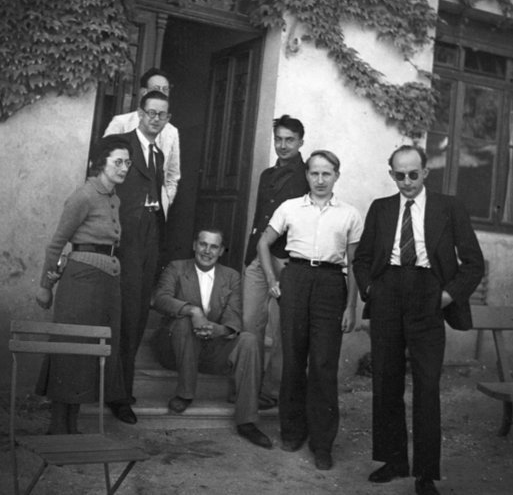
\includegraphics[width=\linewidth]{Bourbaki_congress1938.png}
Bourbaki in Dieulefit\end{minipage}
        }[7]
Let $p$ be a prime of good reduction for $X$ assume we have a \(\QQ_p\)-linear assignment \(\int_b^x :\Omega_{X}^1\otimes \QQ_p \to \QQ_p\) for which:
\[\diff \circ \int_b^x = \mathrm{id},\quad\text{``FTC''}\]%
\[\int_b^x\circ\diff = \mathrm{id}\]%
let $J = \operatorname{Jac}(X)$
% https://q.uiver.app/?q=WzAsNSxbMCwwLCJYKFxcbWF0aGJmIFEpIl0sWzEsMCwiWChcXG1hdGhiZiBRX3ApIl0sWzAsMSwiSihcXG1hdGhiZiBRKSJdLFsxLDEsIkooXFxtYXRoYmYgUV9wKSJdLFsyLDEsIkxpZSBKIChRKSJdLFswLDEsIiIsMCx7InN0eWxlIjp7InRhaWwiOnsibmFtZSI6Imhvb2siLCJzaWRlIjoidG9wIn19fV0sWzAsMiwiIiwyLHsic3R5bGUiOnsidGFpbCI6eyJuYW1lIjoiaG9vayIsInNpZGUiOiJ0b3AifX19XSxbMSwzLCIiLDAseyJzdHlsZSI6eyJ0YWlsIjp7Im5hbWUiOiJob29rIiwic2lkZSI6InRvcCJ9fX1dLFsyLDMsIiIsMix7InN0eWxlIjp7InRhaWwiOnsibmFtZSI6Imhvb2siLCJzaWRlIjoidG9wIn19fV0sWzEsNF0sWzMsNF1d
\[\begin{tikzcd}
	{X(\mathbf Q)} & {X(\mathbf Q_p)} \\
    {J(\mathbf Q)} & {J(\mathbf Q_p)} & {\operatorname{Lie} J (\mathbf Q_p)}
	\arrow[hook, from=1-1, to=1-2]
	\arrow[hook, from=1-1, to=2-1]
	\arrow[hook, from=1-2, to=2-2]
	\arrow[hook, from=2-1, to=2-2]
	\arrow[from=1-2, to=2-3]
	\arrow[from=2-2, to=2-3]
\end{tikzcd}\]
We have
\[\overline {J(\mathbf Q)} \cap X(\mathbf Q_p) \supseteq X(\mathbf Q)\]
now if \[r = \operatorname{rank}(J(\mathbf Q)) < g\] then this intersection is finite!
If we can compute these logarithm functions we can potentially find the intersection explicitly

\emph{Problem:} There are too many functions satisfying all the conditions above, so computing one of them on the nose is hard

\emph{Coleman's idea:} impose that the integral pullback along rigid analytic maps, including for a chosen lift of Frobenius
\[\int_b^x \phi^*\omega = \phi^*\int_b^x \omega\,\quad\text{``Frobenius equivariance''}\]%

We \emph{can} compute the abelian integrals needed for Chabauty by multiplying points on our curve till they lie in the same residue disk on the Jacobian.
%Either we multiply by a very large number (gcd of all possible orders of abvars)

But we would also like for some applications to compute iterated integrals, using Coleman integrals as coefficient functions for 1-forms and iterating again.

To do this, we cannot allow arbitrary rigid functions on our space, but must remove a finite union of disks and consider overconvergent functions:

   \InsertBoxR{0}{\begin{minipage}{0.31\linewidth}
           \centering
           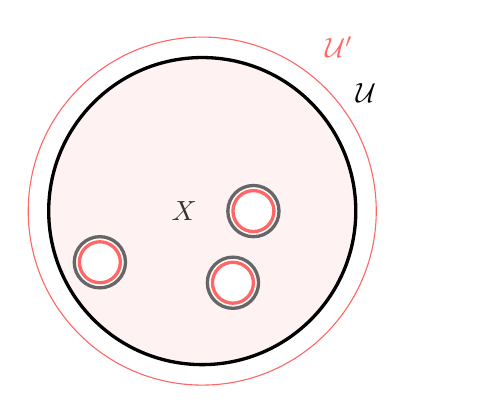
\begin{tikzpicture}[scale=1.3]
               \filldraw[color=black, fill=red!5, very thick](0,0) circle (1.5);
               \node[text width=1.3cm,color=red!60] at (1.7,1.6) {$\mathcal U'$};
               \draw[color=red!60](0,0) circle (1.7);
               \node[text width=1.3cm,color=black] at (2.0,1.15) {$\mathcal U$};
               \filldraw[color=black!60, fill=white, very thick](0.5,0) circle (0.25);
               \filldraw[color=red!60, fill=white, very thick](0.5,0) circle (0.20);
               \filldraw[color=black!60, fill=white, very thick](0.3,-0.7) circle (0.25);
               \filldraw[color=red!60, fill=white, very thick](0.3,-0.7) circle (0.20);
               \filldraw[color=black!60, fill=white, very thick](-1,-0.5) circle (0.25);
               \filldraw[color=red!60, fill=white, very thick](-1,-0.5) circle (0.20);
               \node[text width=1.3cm,color=black!80] at (0.2,0.0) {$X$};
           \end{tikzpicture}
       \end{minipage}%
   }[7]

For example in this way $p$-adic polylogarithms may be defined

$$
\polylog_n (z) = \int \polylog_{n-1}(z) \frac{\diff z}{z},\, \polylog_1(z) = -\log(1-z)
$$

Algorithms to compute these are due to Besser and de Jeu.



\emph{Applications of this theory:}

Coleman integration can be used to define $p$-adic regulators, $p$-adic heights, $p$-adic periods.

Of these, $p$-adic heights have played a big role in the huge effort of several authors that enables the non-abelian Chabauty of Kim to be made effective and computable, some highlights:

\begin{theorem}[Balakrishnan–Dogra–M\"uller–Tuitman–Vonk]
    The (non-)split Cartan modular curve of level 13 is a genus 3 curve which can be given as
    \[\begin{aligned}
        X_s (13) \colon  &y^{4}+5 x^{4}-6 x^{2} y^{2}+6 x^{3} z+26 x^{2} y z+10 x y^{2} z- \\
&10 y^{3} z-32 x^{2} z^{2}-40 x y z^{2}+24 y^{2} z^{2}+32 x z^{3}-16 y z^{3}=0
    \end{aligned}\]
its Jacobian has rank 3, and Picard rank 3.
Then quadratic Chabauty shows that there are exactly 7 rational points on this curve.
\end{theorem}

\begin{theorem}[Balakrishnan--B.--Bianchi--Lawrence--Müller--Triantafillou--Vonk]
The number of rational points on the Atkin--Lehner quotient modular curves $X_0(N)^+ := X_0(N)/w_N$, all of genus 2, rank 2 and Picard rank 2 for $N\in \{67, 73, 103\}$ are as follows:
\[ \#X_0(67)^+(\QQ) = 10,\quad \#X_0(73)^+(\QQ) = 10,\quad \#X_0(103)^+(\QQ) = 8.\]
\end{theorem}

This involves non-abelian Chabauty and Mordell--Weil sieving at $31$ and $137$ in the $N=67$ case.

\begin{theorem}[Balakrishnan–Dogra–M\"uller–Tuitman–Vonk]
The non-split Cartan modular curve of level 17 is a genus 6 curve, its Jacobian has rank 6.
Quadratic Chabauty shows that there are exactly 7 rational points on this curve.
\end{theorem}

Many authors by now use quadratic Chabauty computations for interesting questions in rational points,
Adžaga, Arul, Beneish, Chen, Chidambaram, Keller, and Wen
Arul and Müller, Chidambaram, Keller, and Padurariu, and more ...
%TODO more


\emph{Anatomy of a $p$-adic integral computation:} after Balakrishnan-Bradshaw-Kedlaya

\begin{enumerate}[itemsep=-5mm]
    \item Pick a lift of the Frobenius map
    \item Compute Frobenius action on $H^1$
    \item Evaluate primitives for at least one point in each disk
    \item Compute integrals between nearby points
    \item Solve a linear system
\end{enumerate}
\begin{table}[h!]
    \begin{tabular}{p{40mm}p{50mm}ll}
        Authors                       & Capabilities                                                 & System     & Runtime \\ \hline
        Balakrishnan-Bradshaw-Kedlaya & Odd hyperelliptic curves / $\QQ_p$                                & Sage       &  $p N^2 g^2$ \\
        Balakrishnan-Tuitman (BT)     & General curves with a map to $\mathbf{P}^1$ / ramified & Magma & $p d _ { x } ^ { 4 } d _ { y } ^ { 2 } \left(N^2+d_x d_y N\right)  $ \\
        B.                            & Superelliptic curves / $\QQ_{p^n}$ (some restriction on $p$)                            & Julia/Nemo & $g^3\sqrt p n N^{5/2}$ \\
        B.-Kaya-Keller(+CMM) (after BT)     & General curves with a map to $\mathbf{P}^1$ / mixed          & Magma      & ????
    \end{tabular}
\end{table}

\emph{Note:} also Chabauty code due to e.g. Stoll, Siksek

In the algorithm of Balakrishnan-Tuitman and BKK we work with almost any plane model of a curve, over a number field $K$, of the form
$$X \colon Q(x,y) = 0.$$
(For now we assume $p$ inert in $K$ and take the completion $K_p \simeq \QQ_{p^n}$)

We consider this together with a map $X \xmapsto{x} \mathbf P^1$.

We work in the ring $R^\dagger/K_p$ of overconvergent $p$-adic functions away from the ramification locus.

Then using prior work of Tuitman we can find a Frobenius lift
$$\phi \colon R^\dagger \to R^\dagger$$
$$x\mapsto x^p$$
$$c \mapsto \sigma (c)\text{ for }c \in \QQ_{p^n},$$
a vector of primitives and the matrix capturing the Frobenius action on cohomology
$$
(\phi ^* \omega _i)_i  = M(\omega _i)_i + \underbrace{(\diff f_i)_i}_{=0} \in H^1_{rig}(X\otimes K_p)\text{.}
$$
these can be computed for a basis $(\omega_i)_i$ of 1-forms $p$-adically integral on the complement of the ramification locus.

Roughly, these algorithms (based on Kedlaya's) approximate the Frobenius lift applied to differentials, then try to iteratively reduce the degree of the resulting series by subtracting appropriately chosen exact differentials.
Generally need to consider many terms!

\emph{Over extension fields:}
In order to integrate over $\QQ_{p^n}$ we start with the known data above.
Assuming we want to integrate between two points of $X(\QQ_{p^n})$.

We define the action of \(\phi \) on \(X(\overline {\QQ}_{p^n})\) via%
\begin{equation*}
\phi (x_0, y_0) = (\sigma \inv (\phi (x) (x_0, y_0)), \sigma \inv (\phi (y)(x_0,y_0)))\text{.}\label{x:men:eqn-pt-act}
\end{equation*}
%
\par
On functions \(f\colon X(\overline{\QQ}_{p^n}) \to \overline{\QQ}_{p^n}\) the action of \(\phi \) is then%
\begin{equation*}
\phi (f)(P) = \sigma f(\phi (P))\text{.}\label{x:men:eqn-fun-act}
\end{equation*}

The action the \(n\)th power of Frobenius on the basis differentials is given by%
\begin{equation*}
\phi ^{*n} (\omega_i)_i  = \sum_{t = n-1,\ldots, 0} \left(\prod_{s=n-1, \ldots, t+1} \phi^s(M)\right)\phi ^{*t}(\diff f_i)_i + \prod_{s = n-1, \ldots, 0}\phi ^s(M) (\omega _i)_i\text{.}\label{x:men:eqn-nth-power-frob-act}
\end{equation*}
so that
\begin{gather*}
\left(1 - \prod_{s = n-1, \ldots, 0}\phi ^s(M)\right) \left(\int_{P}^{Q}\omega _i \right)_i = \label{g:mrow:idm445039011104}\\
\left(\int_P^{\phi ^{n}P} \omega _i\right)_i+ \left(\int_{\phi ^{n} Q}^Q \omega _i\right)_i         + \sum_{t = n-1,\ldots, 0} \left(\prod_{s=n-1, \ldots, t+1} \phi^s(M)\right)\sigma^t\left(f_i(\phi ^t Q) - f_i(\phi ^t P)\right)_i\text{.}\label{x:mrow:eqn-final-linear}
\end{gather*}
\par

   \InsertBoxR{0}{\begin{minipage}{0.31\linewidth}
           \centering
           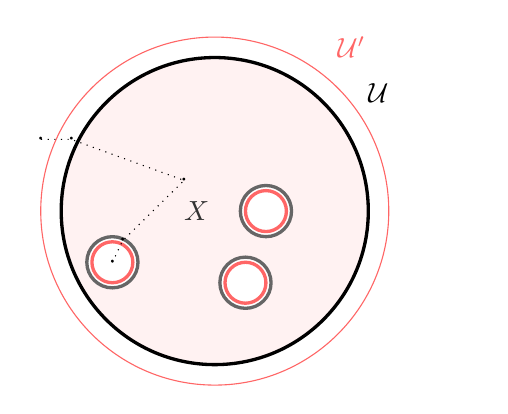
\begin{tikzpicture}[scale=1.3]
               \filldraw[color=black, fill=red!5, very thick](0,0) circle (1.5);
               \node[text width=1.3cm,color=red!60] at (1.7,1.6) {$\mathcal U'$};
               \draw[color=red!60](0,0) circle (1.7);
               \node[text width=1.3cm,color=black] at (2.0,1.15) {$\mathcal U$};
               \filldraw[color=black!60, fill=white, very thick](0.5,0) circle (0.25);
               \filldraw[color=red!60, fill=white, very thick](0.5,0) circle (0.20);
               \filldraw[color=black!60, fill=white, very thick](0.3,-0.7) circle (0.25);
               \filldraw[color=red!60, fill=white, very thick](0.3,-0.7) circle (0.20);
               \filldraw[color=black!60, fill=white, very thick](-1,-0.5) circle (0.25);
               \filldraw[color=red!60, fill=white, very thick](-1,-0.5) circle (0.20);
               \node[text width=1.3cm,color=black!80] at (0.2,0.0) {$X$};
               \draw[dotted] (-1,-0.5) node  {$\cdot$} -- (-0.9,-0.29) node  {$\cdot$} -- (-0.3,0.3) node  {$\cdot$}-- (-1.4,0.7) node  {$\cdot$}-- (-1.7,0.7)node  {$\cdot$};
           \end{tikzpicture}
       \end{minipage}%
   }[7]

As we can compute the RHS and the matrix $M$ we can compute the integrals of basis differentials.

The primitives $f_i$ must be evaluated at at least one point in each disk, and at Frobenius images of these points.

This forces us to pass to a totally ramified extension on top of the unramified one we started with.
We simply choose $\phi$ to be an element of the Galois group of this extension that extends the usual Frobenius on the unramified extension.

In the algorithm for superelliptic curves the superelliptic automorphism is used to conclude that integrals between the bad points all vanish and avoid passing to additional ramified extensions.


\emph{Conclusion:} The algorithm of Balakrishnan-Tuitman can be extended to completely general $p$-adic fields, but remains quite time consuming.

We have a working implementation, and will soon release a preprint with proofs of correctness and complexity analysis.
The Coleman integral is Galois equivariant, which is convenient to check that the implementation is correct, but doesn't seem to help yet when computing.
%\emph{Remark:} This coincides with other forms of $p$-adic integration, such as Colmez's.

Do you have interesting examples for us (curves over $\QQ(\sqrt{-163}) $)!?


\emph{Time for something completely different:}
A Wieferich prime is one for which
$$2^{p-1} \equiv 1 \pmod{p^2},$$
only 2 are known, unlikely $p$-adic closeness.

Katz (2015) reinterprets this as the fact that $2^{\#\mathbf G_m(\mathbf F_p)}$ is closer to the identity $p$-adically than it is forced to be.

If we assume that this happens no more often that it would randomly we get a heuristic for the distribution of Wieferich primes.

Generalizing we consider an abelian variety $A$ and select an integral model of the Lie algebra of the Neron model and a point $P$ of infinite order, consider
\begin{equation*}
    W_P \colon \{p : p\text{ prime},\, p\text{ good}\} \to \LLie(\mathcal A/\ZZ) \otimes_\ZZ (\RR/\ZZ) \cong (\RR/\ZZ)^d\\
\end{equation*}
\begin{equation*}
    p \mapsto\left(\left(\int^{\#\mathcal A_{\mathbf F_p}(\FF_p)P}_0 \omega _i\right)/p \mod p\right)_i
\end{equation*}
we call this quantity $W_P(p)$ the \emph{Wieferich quotient}, the ``first digit'' of the integral.

Katz conjectures that as long as $P$ generates a Zariski dense subgroup, if we take larger $p$ the Wieferich quotients equidistribute.

The genus 2 curve
\begin{equation*}
X\colon  y^2 = 4x^5 - 8x^4 + 8x^3 - 4x^2 + 1
\end{equation*}
\href{https://www.lmfdb.org/Genus2Curve/Q/997/b/997/1}{997.b.997.1}, has a rational point \(x = (0,1)\) such that the class \(P = \lb x - \infty \rb \in \Jac(X)(\QQ)\) is of infinite order.
A histogram of Wieferich quotients of the Coleman integrals of invariant 1-forms is as follows:

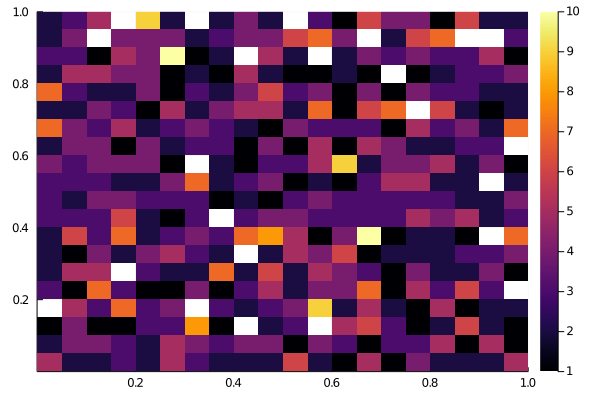
\includegraphics[width=0.9\linewidth]{997.png}

for the Wieferich quotients \(W_P(p)\) for all primes \(15 \lt  p \lt  10000\), and \(p \ne 997\).%

However for the genus 2 curve%
\begin{equation*}
X\colon  y^2 = 4x^5 - 8x^4 + 8x^3 - 4x^2 + 1
\end{equation*}
\href{https://www.lmfdb.org/Genus2Curve/Q/2080/a/4160/2}{2080.a.4160.2}, with \(P = \lb (0,1) - \infty \rb \in \Jac(X)(\QQ)\) of infinite order, the Wieferich quotients \(W_P(p)\) for all primes \(15 \lt  p \lt  10000\).

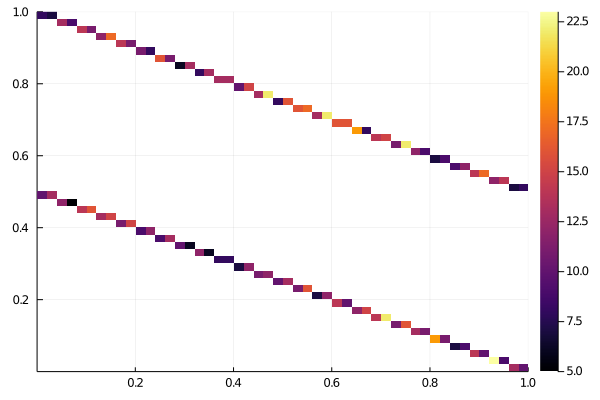
\includegraphics[width=0.9\linewidth]{2080.png}

This curve has Jacobian over \(\QQ\) isogenous the product of elliptic curves 32.a and 65.a. As 32.a is rank 0, the point \(P\) will not generate a Zariski dense subgroup of the Jacobian in this case.%

We see that the annihilating differential is (mod $p$)
\begin{equation*}
\frac{\diff x}{y} +  2x\frac{\diff x}{y}
\end{equation*}
for all these $p$, so almost certainly a global annihilating differential.

Doing these computations type of we gain some evidence for Katz's conjecture, even in cases where other things might interfere, e.g. CM.


\vspace{100em}
\subsection{A worked example}
%\InsertBoxR{0}{\begin{minipage}{0.33\linewidth}
%            \centering
%\begin{tikzpicture}[scale=0.8]
%  \begin{axis}[hide axis]
%    \addplot +[no markers,
%      raw gnuplot,
%      ultra thick,
%      empty line = jump, % not strictly necessary, as this is the default behaviour in the development version of PGFPlots
%      id = grank1,
%      ] gnuplot {
%      set contour base;
%      set cntrparam levels discrete 0.003;
%      unset surface;
%      set view map;
%      set samples 700;
%      set isosamples 500;
%  splot y^2+ (x^3 + x + 1)*y +x^2 + x; };
%  \end{axis}
%\end{tikzpicture}
%        \end{minipage}}[3]%
%        \vspace{1em}
%
%    The genus 2 curve with smallest conductor and positive rank is conjecturally given by
%    \[X \colon y^2 + (x^3 + x + 1)y = -x^2 - x\]
%    Taking $P = (0, -1)$, $b = \infty^+$ we can integrate
%    \[\int^b_P \frac{\diff x }y = -79\cdot3 + O(3^{14}) ,\, \int^b_P \frac{x\diff x }y =  -7010\cdot3^3 + O(3^{14})\]
%    hence
%    \[\int^b_P  (-7010\cdot3^3 + 79\cdot3 x )\frac{\diff x }y  = O(3^{14})\]
%    so any other rational point $Q \in X(\mathbf Q)$ will also have the property that
%    \[\int^b_Q  (-7010\cdot3^3 + 79\cdot3 x)\frac{\diff x }y  = O(3^{14})\]
%    $p$-adically locally this integral can be expressed as a power series in a local parameter $t$.
%    Near $(0,1) \in X(\mathbf Q)$ we may take $t =x $ and calculate the integrals to be:
%    \begin{align*}
%        \int^b_{Q(t)} \omega =& O(3^{15}) + (7010\cdot3^3 + O(3^{14}))\cdot t + (797122\cdot3 + O(3^{14}))\cdot t^2 + (126101 + O(3^{13}))\cdot t^3 \\ & - (382828\cdot3^2 + O(3^{15}))\cdot t^4 + (356687\cdot3^2 + 
%        O(3^{15}))\cdot t^5 - (576544\cdot3 + O(3^{14}))\cdot t^6 \\ & + (54032\cdot3^3 + O(3^{16}))\cdot t^7 + (1162\cdot3^6 + O(3^{14}))\cdot t^8 - (130775\cdot3^{-1} + O(3^{12}))\cdot t^9 \\&+ 
%        (158450\cdot3^2 + O(3^{14}))\cdot t^{10} + (352786\cdot3 + O(3^{14}))\cdot t^{11} + (432610\cdot3^2 + O(3^{15}))\cdot t^{12} \\ &- (167738\cdot3^4 + O(3^{16}))\cdot t^{13} + (701429\cdot3^3 + O(3^{16}))\cdot t^{14} + O(t^{15})
%\end{align*}
%    \InsertBoxR{0}{\begin{tikzpicture}[scale=2]
%	\draw[->] (-0.2,0) -- (2.2,0) node[right] {$i$};
%    \draw[->] (0,-0.1) -- (0,1.6) node[above] {$v_p(a_i)$};
%    \filldraw[black] (0.1,0.4) circle (1pt) node[anchor= south east] {(1,4)}; \filldraw[black] (0.2,0.3) circle (1pt) node[anchor= south west] {(2,3)}; \filldraw[black] (0.3,0.3) circle (1pt) node[anchor= north west] {(3,3)}; \filldraw[black] (0.9,0.8) circle (1pt) node[anchor= south east] {(9,8)}; \filldraw[black] (1.2,1.4) circle (1pt) node[anchor= south east] {(12,14)};
%	%\filldraw[black] (0,0) circle (1pt) node[anchor= north east] {(0,0)};
%    \end{tikzpicture}}[6]
%    As we are looking for roots near $(0,1)$ we can substitute $t = pt$ and find the roots of the resulting series.
%    The roots of this series are
%    \[  O(3^{12}),\,-106289 + O(3^{12}),\,-182670 + O(3^{12}) \]
%    which give $x$-coordinates $0$, $-12/5$, and some wild looking $p$-adic number!
%    We can verify that $0$, $-12/5$ are indeed coordinates of points on the curve.

%    We see from this example that things work best when we have a rational point in each \emph{residue disk}, which we can recover as the root 0 and then have no other roots.


%   \InsertBoxR{0}{\begin{minipage}{0.31\linewidth}
%           \centering
%           \begin{tikzpicture}[scale=1.3]
%               \filldraw[color=red!60, fill=red!5, very thick](0,0) circle (1.5);
%               \node[text width=1.3cm] at (1.7,1.6) {$\mathcal D'$};
%               \draw[color=black](0,0) circle (1.7);
%               \node[text width=1.3cm,color=red] at (2.0,1.15) {$\mathcal D$};
%               \filldraw[color=black!60, fill=white, very thick](0.5,0) circle (0.25);
%               \filldraw[color=red!60, fill=red!60, very thick](0.5,0) circle (0.01);
%               \filldraw[color=black!60, fill=white, very thick](0.3,-0.7) circle (0.25);
%               \filldraw[color=red!60, fill=red!60, very thick](0.3,-0.7) circle (0.01);
%               \filldraw[color=black!60, fill=white, very thick](-1,-0.5) circle (0.25);
%               \filldraw[color=red!60, fill=red!60, very thick](-1,-0.5) circle (0.01);
%               \node[text width=1.3cm,color=black!80] at (0.2,0.0) {$\mathcal V$};
%               \filldraw[color=black, fill=black, very thick](-1.5,-1.1) circle (0.02);
%               \filldraw[color=black, fill=black, very thick](1.75,-0.13) circle (0.02);
%               \filldraw[color=black, fill=black, very thick](-0.75,1.80) circle (0.02);
%               \filldraw[color=black, fill=black, very thick](-0.65,1.70) circle (0.02);
%               \filldraw[color=black, fill=black, very thick](1.8,-1.84) circle (0.02);
%           \end{tikzpicture}
%       \end{minipage}%
%   }[7]

\subsection{Coleman's work}
The above approach is known as \emph{effective Chabauty} and is due to Coleman.
Coleman described how to compute these integrals using \emph{analytic continuation along Frobenius} and proved the following theorem
\begin{theorem}[Coleman's effective Chabauty]
    If $p > 2g$ then
    \[
        | X(\mathbf Q)| \le | X(\mathbf F_p)| + 2g - 2
    \]
\end{theorem}
The proof goes over each disk, estimating the number of zeroes of the integral on each disk.

This bound is sometimes sharp! For instance:

\InsertBoxR{0}{\begin{minipage}{0.35\linewidth}
            \centering
        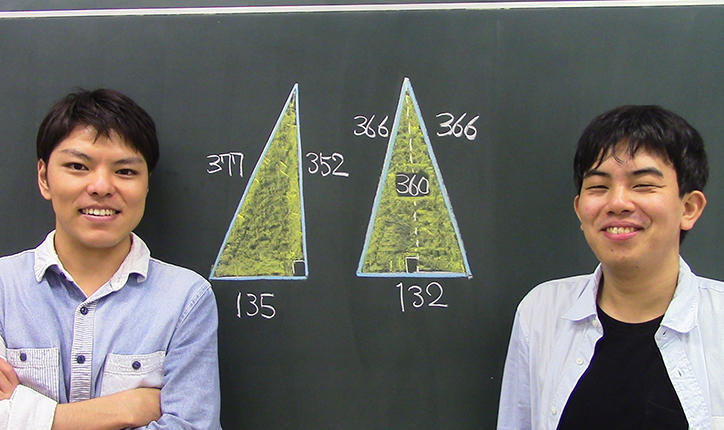
\includegraphics[width=\linewidth]{pic_10.jpg}\end{minipage}
        }[0]
\begin{minipage}{0.60\linewidth}\begin{theorem}[Hirakawa--Matsumura]
There exists a unique pair of a rational right triangle, and a rational isosceles triangle with equal areas and equal perimeters.
\end{theorem}
\begin{proof}
    The problem reduces to finding rational points on the genus 2 rank 1 curve
    \[r^2 = (-3w^2 + 2w^2 - 6w +4)^2 - 8w^6.\]
    which has good reduction at 5, and 8 points over \(\FF_5\).
    Moreover we can find 10 rational points, most of which do not correspond to non-degenerate triangles.
\end{proof}\end{minipage}

Nevertheless it is still often necessary to actually compute these integrals.

\subsection{Computing Coleman integrals}
Coleman's theory makes use of a \emph{lift of Frobenius}, an analytic morphism of an affine curve over $\mathbf Q_p$ that reduces to the Frobenius morphism over $\mathbf F_p$.
\begin{example}
    For \[X \colon  y^2 = f(x)\] a hyperelliptic curve, we can take
    \(\phi \colon x \mapsto x^p\)
    which forces
    \[ (\phi (y))^2 = f (x^p) = f(x^p) - f(x)^p + f(x)^p = f(x^p) - f(x)^p + y^{2p}\]
    hence
    \[ \phi (y) = y^p\sqrt{1 + \frac{f(x^p) - f(x)^p}{y^p}}\]
    on the locus away from $y = 0$.
\end{example}

The property of Coleman integrals that makes the theory uniquely defined, is that we ask the integrals to be equivariant for some (any) lift of Frobenius.


    %Throughout we take \(X/\ZZ_p\) a genus \(g\) odd degree hyperelliptic curve, and \(p\) an odd prime.
    We pick a lift of the Frobenius map, on some affine subvariety $A$ of $X$, \(\phi^*\colon A \to A\), and write \(A^\dagger\) (resp.\ \(A_{\text{loc}}(X)\)) for overconvergent (resp.\ locally analytic) functions on \(A\).
    \begin{theorem}[{Coleman}]
        There is a (unique) \(\QQ_p\)-linear map \(\int_b^x\colon \Omega_{A^\dagger}^1\otimes \QQ_p \to A_\mathrm{loc} (X)\) for which:\leavevmode%
        \[\diff \circ \int_b^x = \mathrm{id}\colon \Omega_{A^\dagger}^1\otimes \QQ_p \to \Omega_{\text{loc}}^1\,\quad\text{``FTC''}\]%
        \[\int_b^x\circ\diff = \mathrm{id}\colon A^\dagger \hookrightarrow A_{\mathrm{loc}}\]%
        \[\int_b^x \phi^*\omega = \phi^*\int_b^x \omega\,\quad\text{``Frobenius equivariance''}\]%
    \end{theorem}

    \begin{itemize}
        \item Balakrishnan--Bradshaw--Kedlaya reduce the problem of computing all Coleman integrals of basis differentials \(\omega_i\) of \(H^1_{\mathrm{dR}}(X)\) between \(\infty\in X\) and a point \(x\in X(\QQ_p)\) on an odd degree hyperelliptic curve, to:
    \begin{enumerate}
        \item Finding ``tiny integrals'' between nearby points,
        \item Writing \(\phi^*\omega_i  - \diff f_i=\sum_j a_{ij}\omega_j \) and evaluating the primitive \(f_i\) for a point \(P\) near \(x\), for each \(i\).
    \end{enumerate}
        \item Balakrishnan--Tuitman gave a more general version of this procedure that works on a very large class of curves.
        \item B. gave a computationally more efficient method for superelliptic curves, using work of Harvey and Minzlaff, that also works over unramified extensions of $\QQ_p$.
    \end{itemize}

    %Applying \(\phi^*\) to the basis \(x^i \diff x/2y\) for \(i = 0,\ldots, 2g-1\) gives
    %\[\phi^* \omega_i \equiv\sum_{j=0}^{N-1} \sum_{r=0}^{(2g+1)j} B_{j,r} x^{p(i+r+1) - 1}y^{-p(2j+1) + 1} \frac{\diff x}{2y}\pmod{p^N}\]
    %\(B_{j,r}\in \ZZ_p\) are in terms of coefficients of the curve and binomial coefficients.



\section{Number field Chabauty}
If we work over a fixed number field $K$ one can make sense of all of the above, and sometimes one can do better following ideas of Siksek and Wetherell.

If $X/K$ is a curve over a number field $K$ of degree $d$ then \(\Res_{K/\QQ} (X)\)
is a $d$-dimensional projective variety such that
\[V = \Res_{K/\QQ} (X)(\QQ) \leftrightarrow X(K)\]
and
\[A = \Res_{K/\QQ} (\Jac(X))\]
is a $gd$-dimensional abelian variety.
Then the analogous Chabauty diagram is
\[\begin{tikzcd}
	{V(\mathbf Q)} & {V(\mathbf Q_p)} \\
    {A(\mathbf Q)} & {A(\mathbf Q_p)} & {\operatorname{Lie} A (\mathbf Q)}
	\arrow[hook, from=1-1, to=1-2]
	\arrow[hook, from=1-1, to=2-1]
	\arrow[hook, from=1-2, to=2-2]
	\arrow[hook, from=2-1, to=2-2]
	\arrow[from=1-2, to=2-3]
	\arrow[from=2-2, to=2-3]
\end{tikzcd}\]
where now
\[\dim \overline{A(\QQ)} = \rank(J(K)),\,
\dim V(\QQ) = d\]

If \(d + r \le gd \) then we might \emph{hope} that the intersection of these two subspaces is finite, and we can therefore cut out $X(K)$ whenever
\(r \le (g - 1)[K : \QQ]\).

%
%\InsertBoxR{0}{
%    \begin{tikzpicture}[scale=3,
%  line cap=but,
%  l/ine join=round,
%  x=.5em,
%  ultra thick,
%  y=1*(height("Z")-\pgflinewidth)*(1-sin(10)),
%  rotate=-10,
%  rounded corners=1.5pt,
%]\draw (1, 0) -- (0, 0) -- (1, 1) -- (0, 1);\end{tikzpicture}}[4]
\begin{warning}
    The intersection is not always finite! This was noted by Siksek, but even Siksek's guess for a sufficient condition also turned out to be false, as shown by Dogra, with the example of a genus 3 hyperelliptic curve over $\QQ(\sqrt{33})$.
\end{warning}

Nevertheless in practice this approach is quite useful, Siksek gives an explicitly checkable condition that can be used to verify that rational points are alone in their residue disk.

\begin{theorem}[Siksek]
    For every $K$-rational point $Q$ of $X/K$ there is an effectively computable matrix $M_p(Q)$ defined using the integrals of holomorphic 1-forms against a basis of a free subgroup of finite index in $J(K)$, and the local behaviour of the basis of 1-forms such that if the reduction of $M_p(Q)$ has rank $d$ then $Q$ is the only $K$-rational point of the curve in a $p$-adic unit ball around $Q$.
\end{theorem}

\begin{example}[B.--Dahmen]
    Consider \(X\colon  x^{13} + y^{13} = z^5\), one of the generalized Fermat curves, then there exists a covering map
    \[X \to C \colon y^2 = 4 x^5 + 1677 \alpha^2 - 2769 \alpha + 637/K\]
    where
    \[K = \QQ(\alpha ) = \QQ[x]/(x^{3} - x^{2} - 4 x - 1)\]
    is the unique cubic subfield of $\QQ(\zeta _{13})$.
    This curve has rank 2 over $K$ and genus 2, so regular Chabauty does not apply.
    Nevertheless Siksek's techniques using the prime $47$ suffice to show that there are only five $K$-rational points on $C$.
\end{example}


\section{Removing extra points -- the Mordell--Weil sieve}
This is a technique that first appears in the work of Scharaschkin, that is extremely useful to rule extra points that appear in the Chabauty method.

In the example above we had a zero of our integrals that didn't appear to correspond to a rational solution.
Once again fixing a rational base point $b\in X(\QQ)$ for simplicity we have:
\[\begin{tikzcd}
	{X(\mathbf Q)} & {J(\mathbf Q)} \\
    {X(\mathbf F_\ell)} & {J(\mathbf F_\ell)}
    \arrow["\AJ",hook, from=1-1, to=1-2]
	\arrow["\red_X",hook, from=1-1, to=2-1]
	\arrow["\red_J", hook, from=1-2, to=2-2]
    \arrow["\AJ_\ell"hook, from=2-1, to=2-2]
\end{tikzcd}\]
where now the image of any rational point lands in the union of cosets $\red_J^{-1}(\AJ_\ell(X(\FF_\ell)))$.

In order to prove non-rationality of certain $p$-adic points we make use of the $p$-adic filtration on $J$, points of $X(\QQ)$ whose difference lies in a group of large $p$-power order of the Jacobian are $p$-adically close on the Jacbian, and hence on the curve itself.

By varying $\ell$ over primes such that a power of $p$ divides $|J(\FF_\ell)|$ we increasingly place restrictions on how $p$-adically close any putative rational point must be to one of our known rational points.

Using just the sieve on its own we always cut out a union of $p$-adic balls, which is infinite if non-empty, but coupled with finiteness from Chabauty we can often determine exactly the set of rational points.


\emph{The question remains, what if $r \ge g$?}


%\section{Elliptic Curve Chabauty}
\section{Chabauty--Kim}
Minhyong Kim has extended the core idea of Chabauty, inspired in part by the \emph{section conjecture} of Grothendieck that
\[X(\mathbf Q) \simeq H^1(G, \pi_1^{\et} (\overline X, b)).\]
Kim considers the $\mathbf Q_p$-pro-unipotent \'etale fundamental group, denoted \(U\), this has a descending central series filtration $U = U^1 \supset U^2 \supset \cdots$, for which the quotients $U_i = U/U^i$ get increasingly non-abelian as $i \gg 1$.
Kim defines local and global \emph{Selmer schemes} that fit into an analogous diagram as before, for each $n$

\[\begin{tikzcd}
    {X(\mathbf Z[1/S])} & {X(\mathbf Z_p)} \\
    {H^1_f(G,U_n)} & {H_f^1(G_p, U_n)} & {U_n^{DR}/F^0}
	\arrow[hook, from=1-1, to=1-2]
	\arrow[from=1-1, to=2-1]
	\arrow[from=1-2, to=2-2]
    \arrow["loc_p",from=2-1, to=2-2]{loc_p}
	\arrow[from=1-2, to=2-3]
	\arrow[from=2-2, to=2-3]
\end{tikzcd}\]

The bottom horizontal maps are algebraic, and the vertical maps are transcendental.

Kim conjectures that for some \emph{depth} $n$ we always have that the image of $loc_p$ is not Zariski dense and so a Chabauty-like argument applies to show finiteness of rational points.
Kim also expects that for $n \gg 1$ this method will cut out precisely the set of rational points, with no extra transcendental points like we had before.

In depth 1 this gives us a diagram which is essentially the original Chabauty diagram.


\subsection{Quadratic Chabauty}
Work of Balakrishnan--Dogra makes Chabauty--Kim more effective in the case that the rank of the Neron--Severi group of the Jacobian is at least 2.
This allows them to find a more approachable quotient of the group $U_2$ and make a connection with $p$-adic heights to get a handle on the functions appearing


\subsection{Applications to modular curves}
\subsection{Integral points and connection with the $S$-unit equation}
In addition to answering questions about rational points, Chabauty techniques can also be used to determine or bound integral points, by considering punctured curves:

Letting $X = \PP^1 \smallsetminus \{0,1,\infty \}$ and fixing a finite set of rational primes $S$ we have
\[X(\ZZ[1/S]) = \{(u,v) \in (\ZZ[1/S]^\times)^2: u+ v = 1 \}\]
the solutions to the \emph{$S$-unit equation}.

The Chabauty diagram in this case involves the \emph{generalised Jacobian}, for a prime $p \not\in S$
\[\begin{tikzcd}
    {X(\mathbf Z[1/S])} & {X(\mathbf Z_p)} \\
    {\GG_m(\mathbf Z[1/S] )^2} & {\GG_m(\mathbf Z_p )^2} & {\ZZ_p^2}
	\arrow[hook, from=1-1, to=1-2]
	\arrow[hook, from=1-1, to=2-1]
	\arrow[hook, from=1-2, to=2-2]
	\arrow[from=2-1, to=2-2]
	\arrow[from=1-2, to=2-3]
	\arrow[from=2-2, to=2-3]
\end{tikzcd}\]
from this we see that the rank $<$ genus condition is almost never satisfied.

But passing to non-abelian Chabauty in depth 2 we obtain the diagram
\[\begin{tikzcd}
    {X(\mathbf Z[1/S])} & {X(\mathbf Z_p)} \\
    {\Aff^{2|S|}} & {\Aff^3}
	\arrow[hook, from=1-1, to=1-2]
	\arrow[hook, from=1-1, to=2-1]
	\arrow[hook, from=1-2, to=2-2]
	\arrow[ from=2-1, to=2-2]
\end{tikzcd}\]

where $\Li_2 (z) = \int \frac{\log (1-w)}{w} \diff w$ is an \emph{iterated Coleman integral}.
Defined near zero by the series
\[\sum_{i=0}^\infty \frac{z^i}{i^2}.\]


The bottom horizontal arrow is more mysterious.
In joint work with Betts--Kumptisch--L\"udtke--McAndrew--Qian--Studnia--Xu we study the $S_3$-equivariance of this set-up.
We also apply \emph{refined non-abelian Chabauty--Kim} to reduce the dimension of the bottom left entry and apply this extension of Chabauty when $|S| = 2$.

\section{Other applications}
\subsection{Integral points}
\subsection{Torsion points}
\section{General fields}
with E. Kaya \& T. Keller

Following Balakrishnan-Tuitman

\end{document}
